
\subsection{Introduction}

\begin{center}
    \textit{Cloud computing is a model for enabling convenient, 
        on-­demand network access to a shared pool of configurable 
        computing resources (e.g., networks, servers, storage, 
        applications, and services) that can be rapidly provisioned 
        and released with minimal management effort or 
    service provider interaction.}
\end{center}

\begin{tabular}{cm{10cm}}
    \textbf{Cloud commandments (eBay)} &
    \begin{enumerate}
        \item Partition everything
        \item Use asynchony everywhere
        \item Automate everything
        \item Remember that everything fails
        \item Embrace inconsistency
    \end{enumerate}
\end{tabular}

\begin{tabular}{cm{10cm}}
    \textbf{Cloud benefit} &
    \begin{itemize}
        \item Elastic, just-­in-­time infrastructure
        \item More efficient resource utilization
        \item Pay for what you use
        \item Potential to reduce processing time (parallelization)
        \item Leverage multiple data centers (high availability)
    \end{itemize}
\end{tabular}


\subsubsection{Hardware scalability}

Cloud need for \textbf{scalability} because modern application require
huge amounts of processing and data. Cluster (\textit{room-sized}) and datacenter 
(\textit{building-sized}) can provide the resources needed.
They are composed of \textbf{rack} which is a aggregation of storage devices, many
nodes and switch to connect nodes together. Unfortunately, they are not perfect.
\begin{enumerate}
    \item Difficult to dimension because they must be provisioning for the peak load
    \item Expensive in hardware invest, expertise (ex: special software) and maintenance
    \item Difficult to scale because adding new machines is not easy
\end{enumerate}


\subsubsection{Model}
Cloud computing is a business models where everything is a service:
\begin{itemize}
    \item \textbf{SaaS} (Software as a service): Soft run on distant server 
        instead on running on the user machine.

        \begin{tabular}{m{5cm}m{10cm}}
        $\Rightarrow$ Customer pay cloud provider
        &
        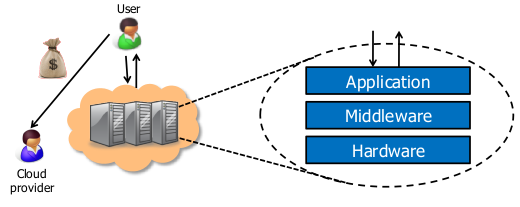
\includegraphics[width=7cm]{img/saas}
        \end{tabular}
        SaaS is like using Dropbox.
    \item \textbf{PaaS} (Platform as a service):  Customers handle the application.

        \begin{tabular}{m{5cm}m{10cm}}
            $\Rightarrow$ Customer pay SaaS provider for service which
            pays cloud for the infrastructure.
        &
        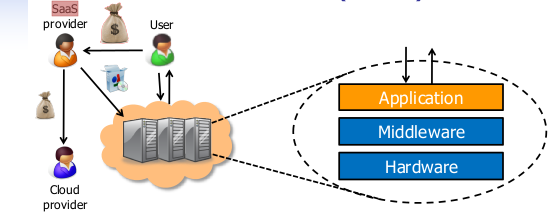
\includegraphics[width=7cm]{img/paas}
        \end{tabular}

        PaaS is like using Hadoop plateform on amazon.
    \item \textbf{IaaS} (Infrastructure as a service): Customers handle the 
        middleware and application. Provider handle hardware.

        \begin{tabular}{m{5cm}m{10cm}}
            $\Rightarrow$ Customer pay SaaS provider for service which
            pays cloud for resources.
        &
        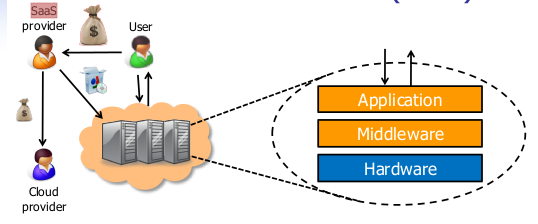
\includegraphics[width=7cm]{img/iaas}
        \end{tabular}

        Only the IaaS have to take in account the scaling model 
        (which tools according to the size of the client). It's like
        using pythonanywhere, or EC2.
\end{itemize}

\subsubsection{Types}
There also have three types of cloud : 
\begin{itemize}
    \item \textbf{Public}: commercial commercial service open to almost anyone.
    \item \textbf{Community}: shared by several similar organization
    \item \textbf{Private}: shared within a organization
\end{itemize}
In this course we focus on public cloud.

\subsubsection{Applications}

Typically, applications that involve large amounts of computation, storage,
bandwidth Especially when lots of resources are needed quickly or load varies
rapidly.

\begin{itemize}
    \item \textbf{Web app}: Near the edge of the application focus is on vast 
        numbers of clients and rapid response
    \item \textbf{Processing pipelines}: Inside we find data-­intensive services that 
        operate in a pipelined manner, asynchronously
    \item \textbf{Batch processing}: Deep inside the application we see a world of 
        virtual computer clusters that are scheduled to 
        share resources and on which applications like 
        MapReduce (Hadoop) are very popular
\end{itemize}


\subsubsection{Virtualization}
It is used to simulate multiple physical machine for the consumer with different
capabilities. It's powerful for security and isolation because VM cannot influence
other and it provides high flexibility. In the other hand, performance is hard 
to predict because other VM run on the same physical machine.

\subsubsection{Challenge}
\begin{tabular}{m{0.5\linewidth}m{0.5\linewidth}}
    \begin{itemize}
        \item Availability
        \item Data lock-in (moving data)
        \item Data confidentiality and auditability 
        \item Data transfer bottlenecks
        \item Performance unpredictability for VM
    \end{itemize}
    &
    \begin{itemize}
        \item Scalable storage
        \item Bugs in large distributed systems
        \item Scaling quickly
        \item Reputation fate sharing
        \item Software licensing
    \end{itemize}
\end{tabular}


